\documentclass[10pt, final, hyperref, table]{beamer}
\mode<presentation>


 %\usepackage[english]{babel} % "babel.sty"
% \usepackage{french}                  % "french.sty"
%  \usepackage{franglais}               % "franglais.sty" (a defaut)
  \usepackage{times}			% ajout times le 30 mai 2003
 
%% --------------------------------------------------------------
%% CODAGE DE POLICES ?
%% Si votre moteur Latex est francise, il est conseille
%% d'utiliser le codage de police T1 pour faciliter la césure,
%% si vous disposez de ces polices (DC/EC)
\usepackage[utf8]{inputenc}
\usepackage[T1]{fontenc}


%% ==============================================================
%\usepackage{graphicx}
\usepackage{amsmath,amsfonts}
%\usepackage[table]{xcolor}
\usepackage{subfigure}
\usepackage{fancybox}

\usepackage{multicol}
\usepackage{wrapfig}
\usepackage{listings}
\usepackage{xcolor}
\usepackage{multimedia} % For playing sound

\usepackage{hyperref}
% Define hyperlinks color
\definecolor{links}{HTML}{2A1B81}
\hypersetup{colorlinks,linkcolor=,urlcolor=links}

\usetheme{Madrid}
\setbeamercovered{transparent}


% telemeta red
\definecolor{telemetaRed}{rgb}{0.41568, 0.01176, 0.02745}	% #6A0307
\usecolortheme[rgb={0.41568, 0.01176, 0.02745}]{structure} 

%\setbeamercolor{frametitle}{bg=telemetaRed}
% Display a grid to help align images
%\beamertemplategridbackground[1cm]

%We will get the normal bibliography style (number or text instead of icon) by including the following code
\setbeamertemplate{bibliography item}[text]
\setbeamerfont{caption}{size=\footnotesize}
% listings settings
\definecolor{lstComments}{rgb}{0,0.6,0}
\definecolor{lstBkgrd}{rgb}{0.95,0.95,1}
\lstset{%
  language=Python, % the language of the code
  frame=single,  % adds a frame around the code
  frameround=tttt,
  commentstyle=\color{lstComments},% comment style
  backgroundcolor=\color{lstBkgrd},   % choose the background color
  basicstyle=\tiny,       % the size of the fonts that are used for the code
  stringstyle=\ttfamily,  % typewriter type for strings
  keywordstyle=\color{blue},      % keyword style
  showstringspaces=false,          % underline spaces within strings only
}
\title[TimeSide]{TimeSide\\\emph{ Open web audio processing framework}}

\author{Thomas Fillon \inst{1,2}, Guillaume Pellerin\inst{1}}


\institute[Parisson]{
  \inst{1}%
  Parisson, Paris, France\\
  \inst{2}%
  LAM, Institut Jean Le Rond d'Alembert, UPMC Univ. Paris 06, UMR CNRS 7190, Paris, France\\
\vskip1ex
 \begin{center}
   
\includegraphics[width=.5\linewidth]{../../Common/img/parisson_logo_FINALE_com.pdf}
 \end{center}
}
\date{IRCAM - WAVE \\ 13/03/2014}        


\newcommand{\pyfile}{$\vcenter{\hbox{
\includegraphics[width=1cm]{img/python-file.png}}}$}
\newcommand{\gstreamer}{\href{http://www.gstreamer.freedesktop.org}{$\vcenter{\hbox{
\includegraphics[width=0.20\textwidth]{img/Gstreamer-logo.png}}}$}}
\begin{document}
\begin{frame}
  \maketitle
\end{frame}

\begin{frame}
 \frametitle{TimeSide - Goals}%\scriptsize
% ==================================
% --------- Résumé -----------------
% ==================================
\begin{block}{Server side - TimeSide Engine}

  \begin{itemize}
  \item \alert{Do} asynchronous and fast audio processing with Python,
  \item \alert{Decode} audio frames from ANY format into numpy arrays,
  \item \alert{Analyze} audio content with state-of-the-art audio feature extraction libraries,
  \item  \alert{Organize}, serialize and save analysis metadata through various formats,
  \end{itemize}
  \end{block}
 \begin{block}{}
    \begin{itemize}
      \item  \alert{Draw} various fancy waveforms, spectrograms and other cool graphers,
  \item  \alert{Transcode} audio data in various media formats and stream them through web apps,

    \end{itemize}
 
\end{block}
\begin{block}{Client side - TimeSide UI}
  \begin{itemize}
  \item   \alert{Playback} and  \alert{interact} on demand through a smart high-level HTML5 extensible player,
  \item   \alert{Index},  \alert{tag} and  \alert{organize semantic metadata} \\
(see \href{http://telemeta.org/}{Telemeta} which embeds TimeSide). 
\hfill $\vcenter{\hbox{
\includegraphics[width=0.2\textwidth]{../../Common/img/logo_telemeta_1-1.pdf}}}$
 % \begin{flushright}
 %   
\includegraphics[width=0.2\textwidth]{../../Common/img/logo_telemeta_1-1.pdf}\\
 %   \colorbox{yellow!50}{\textbf{\url{http://telemeta.org/}}}
  %\end{flushright}
  \end{itemize}
\end{block}
\end{frame}

\begin{frame}
  \frametitle{TimeSide Engine Architecture}
  \begin{center}
    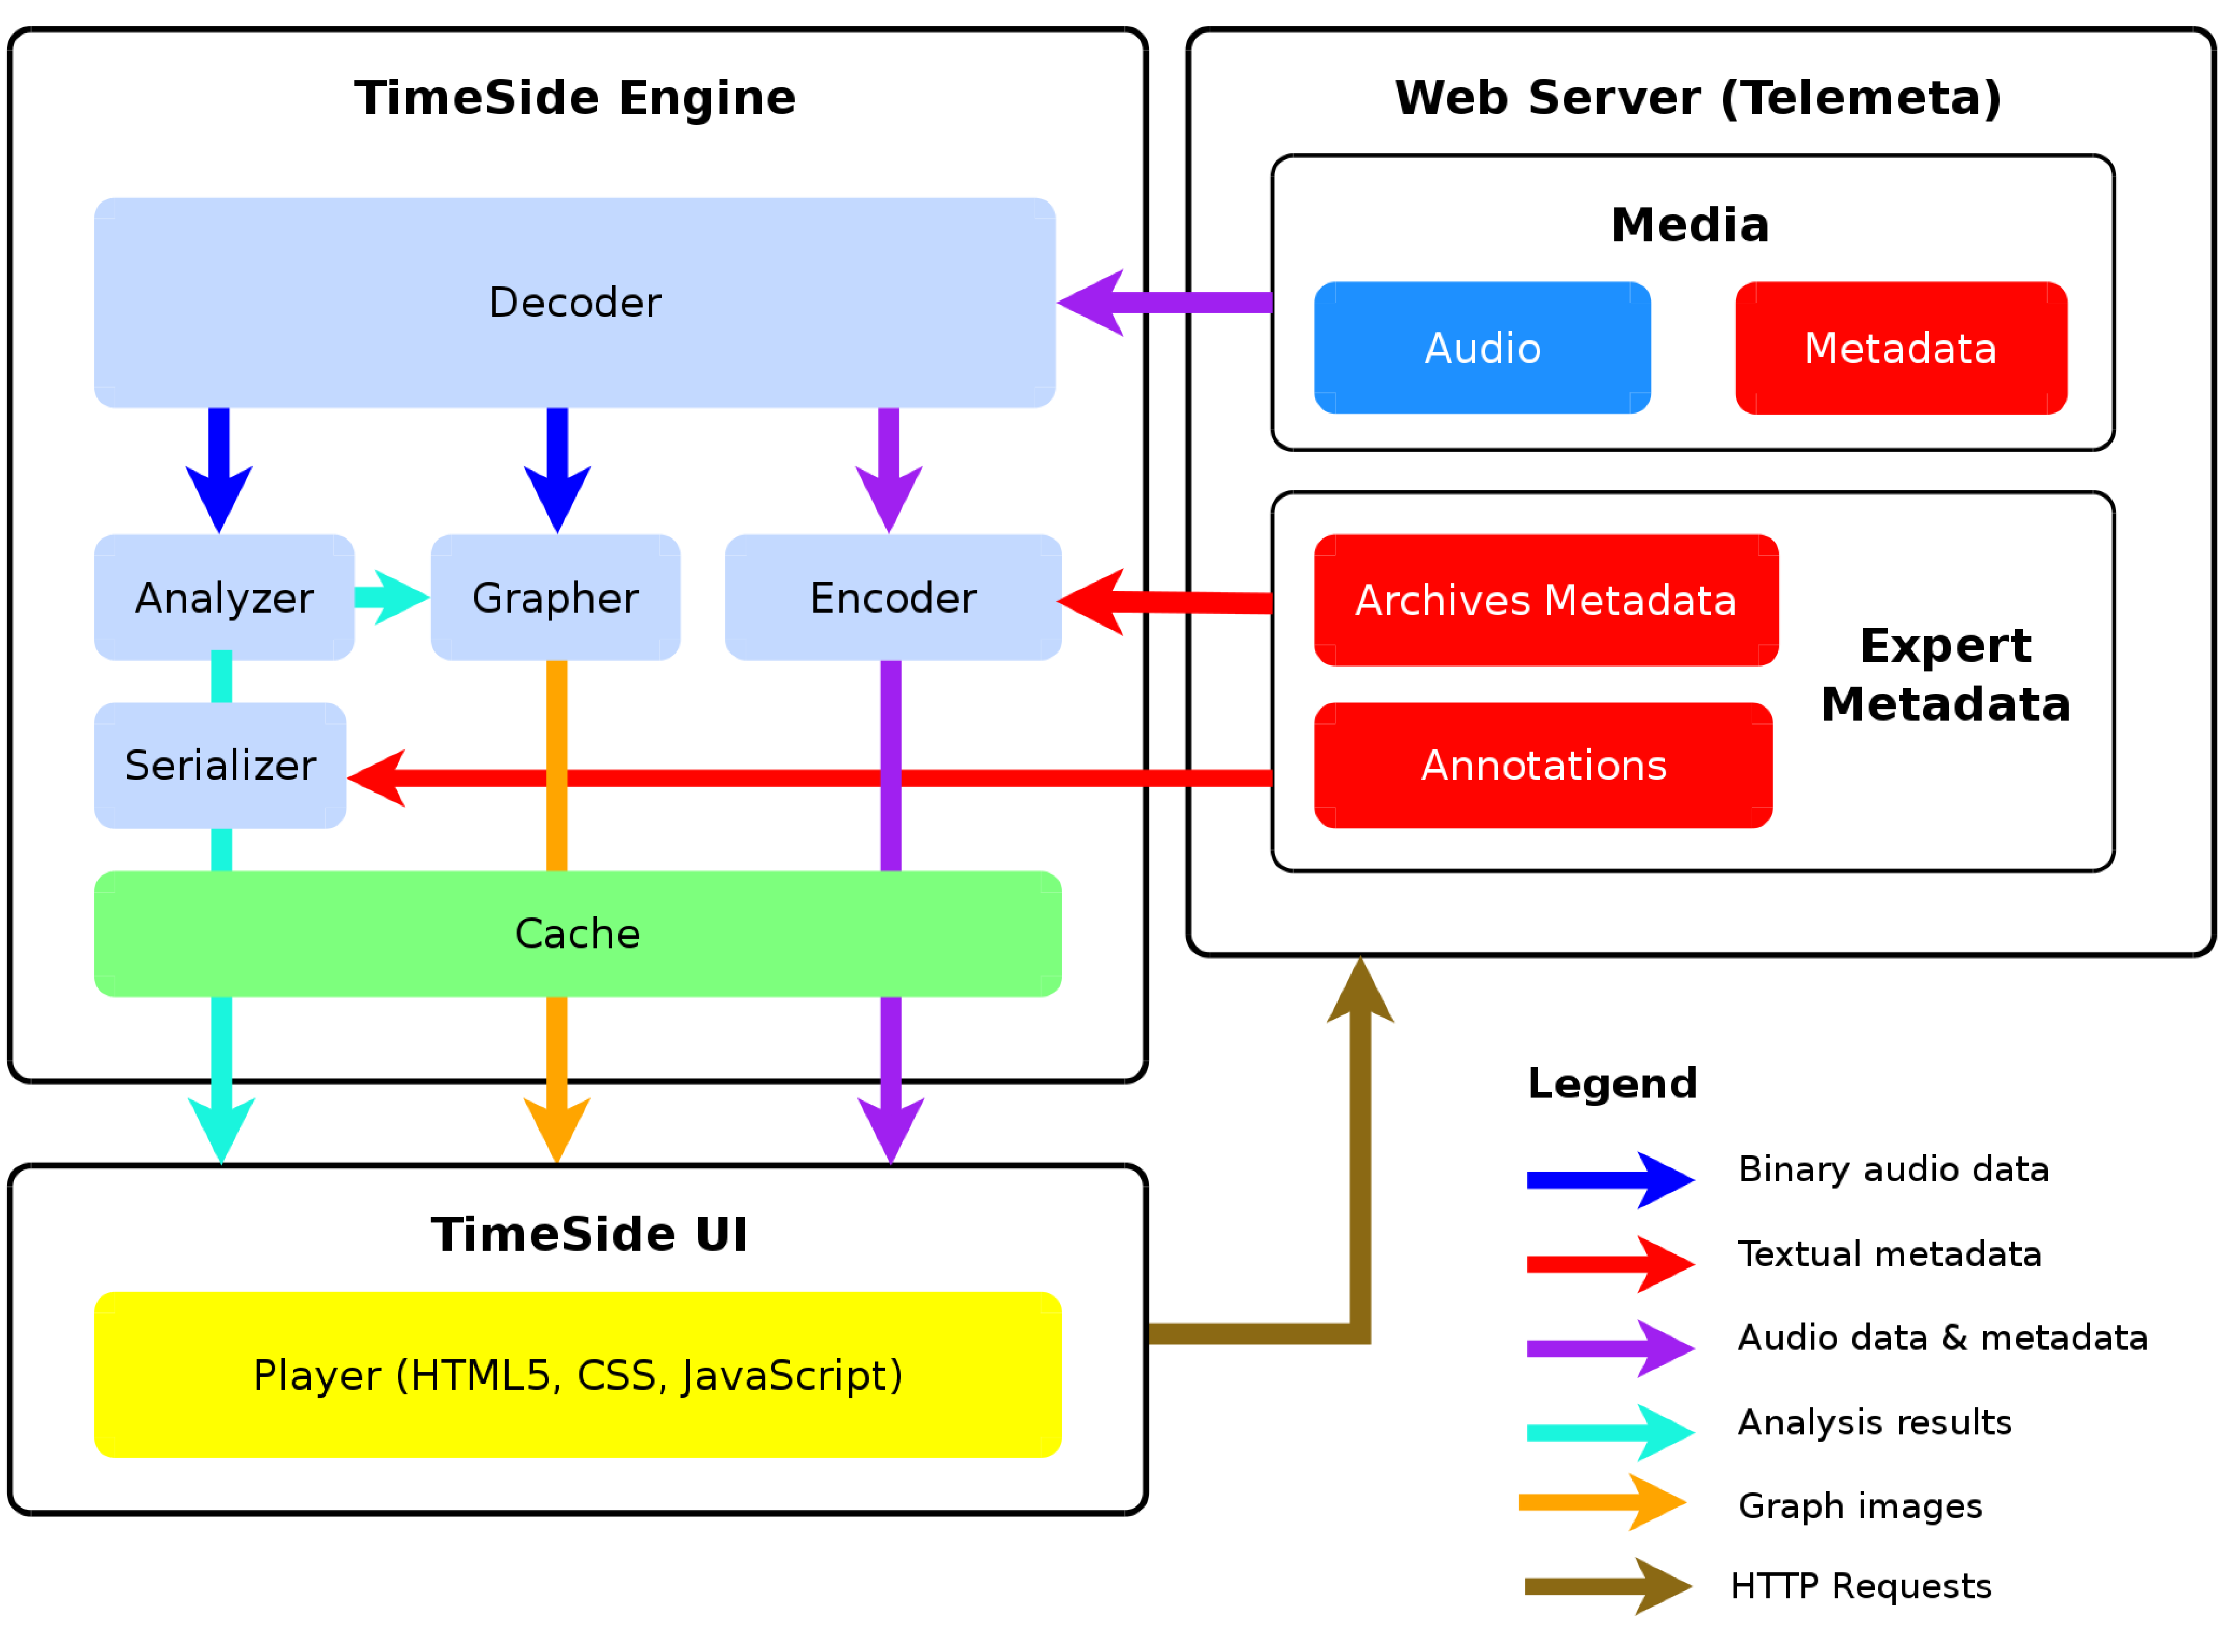
\includegraphics[width=0.8\textwidth]{../../Common/img/timeside_schema_v3.pdf}
  \end{center}
\end{frame}
\begin{frame}
  \frametitle{Processors}
  \begin{block}{4 types of processors}
    \begin{itemize}
    \item Decoder
    \item Analyzer
    \item Encoder
    \item Grapher
    \end{itemize}
  \end{block}
\pyfile : \texttt{timeside/api.py}, \texttt{timeside/core.py}
\end{frame}

\begin{frame}
  \frametitle{Processors - Decoders}
  \begin{block}{Decoders}
    \begin{itemize}
    \item FileDecoder: Decode audio through Gstreamer \gstreamer
      
      \begin{itemize}
      \item File source: an \texttt{uri}
      \item A \alert{segment} of audio can be specified: \texttt{start, duration}
      \end{itemize}

    \item \alert{ArrayDecoder}: Use an Numpy array as source input
    \item \alert{LiveDecoder}: Capture audio from an live input source
    \end{itemize}
  \end{block}
\pyfile : \texttt{timeside/decoder/core.py}, \texttt{timeside/decoder/file.py} 
\end{frame}

\begin{frame}
  \frametitle{Processors - Encoders}
  \begin{block}{Encoders}
    \begin{itemize}
    \item Support streaming to the server
    \item Available formats (through Gstreamer) \gstreamer

      \begin{itemize}
      \item WavEncoder, FlacEncoder
      \item AacEncoder, VorbisEncoder, Mp3Encoder
      \item WebMEncoder, \alert{OpusEncoder}
      \item LiveEncoder : Send sound to soundcard
      \end{itemize}
    \end{itemize}

  \end{block}
\pyfile : \texttt{timeside/encoder/core.py}, \texttt{timeside/encoder/mp3.py} 
\end{frame}

\begin{frame}
  \frametitle{Processors - Analyzers}
    \begin{block}{Analyzers}
      \begin{itemize}
      \item Value Analyzers: Level, MeanDCShift
      \item \alert{Wrapping of \emph{state-of-the-art} audio features library}:
\begin{itemize}
\item Aubio: \colorbox{yellow!50}{\hskip1ex  \url{http://aubio.org} \hskip1ex }\\
AubioTemporal, AubioPitch, AubioMfcc, AubioMelEnergy, AubioSpecdesc
\item Yaafe: \colorbox{yellow!50}{\hskip1ex \url{http://yaafe.sourceforge.net}\hskip1ex }
\item Vamp plugins: \colorbox{yellow!50}{\hskip1ex \url{http://www.vamp-plugins.org}\hskip1ex } VampSimpleHost
\end{itemize}
        \item \alert{Waveform}, \alert{Spectrogram}
      \item Speech Activity Detection: \alert{IRITSpeechEntropy}, \alert{IRITSpeech4Hz}, LimsiSad
      \item \alert{OnsetDetectionFunction}
      \end{itemize}
    \end{block}
    \alert{$\rightarrow$ An analyzer can declare other analyzers as \emph{parents}}
    
\pyfile :  \texttt{timeside/analyzer/core.py}, \texttt{timeside/analyzer/odf.py} 
  \end{frame}
\begin{frame}
  \frametitle{Processors - Graphers}
    \begin{block}{Graphers}
      \begin{itemize}
      \item Waveform
      \item WaveformCentroid 
      \item \alert{WaveformTransparent}
      \item WaveformContourBlack
      \item WaveformContourWhite
      \item SpectrogramLog
      \item \alert{SpectrogramLinear} 
      \end{itemize}
    \end{block}
 \alert{$\rightarrow$ Possibility to define grapher from analyzer}
  \end{frame}
\begin{frame}
  \frametitle{Principales nouveautés}
  \begin{block}{}
    \begin{itemize}
    \item Version 0.5.4 
    \item Mise en place d'une documentation :
      \url{http://files.parisson.com/timeside/doc/}
   
    \item Installation par paquets Debian (Timeside + Aubio + Yaafe)
      pour Debian Stable 7.0 Wheezy
      \url{https://github.com/yomguy/TimeSide\#install}
    \item Outil en \emph{ligne de commande} : \texttt{timeside-launch}
    \item Décodeur : possibilité de lire un \alert{segment} de fichier audio
    \end{itemize}
  \end{block}
  \begin{block}{Analyseurs - Sauvegarde des résultats}
    \begin{itemize}
    \item Amélioration de la sérialisation des resultats (xml, json,
      yaml, \alert{numpy}, \alert{hdf5})
    \item  Ajout de fonctionnalités et \emph{Réusinage} de code en prévision de l'intégration de méthodes d'analyse automatique
    \item Notion d'analyseur " \emph{parent} "
    \end{itemize}
    
  \end{block}
\end{frame}

\begin{frame}{Analyzer results container}
\begin{block}{Results types}
  Standardization of 8 different types of results:
  \begin{itemize}
  \item time\_mode : \texttt{global, event, segment, framewise}
  \item data\_mode : \texttt{value, label}
  \end{itemize}
\end{block}
\begin{block}{Metadata \& Data fields}
  \begin{itemize}
  \item Metadata:
    \begin{itemize}
    \item \texttt{id\_metadata}
    \item \texttt{audio\_metadata}
    \item \texttt{label\_metadata}
    \item \texttt{frame\_metadata}
    \item \texttt{parameters}
    \end{itemize}
    \item Data: \texttt{data\_object}
  \end{itemize}

\end{block}

\end{frame}

\begin{frame}[fragile]
  \begin{block}{TimeSide - Github repository}
    \begin{center}\scriptsize
      \colorbox{yellow!50}{\bf \hskip3ex
        \url{https://github.com/yomguy/TimeSide/} \hskip3ex }
    \end{center}

  \begin{itemize}
  \item 3 main branches: master (0.5.2), dev, diadems 
  \end{itemize}
  \end{block}
  \begin{block}{Installation}
\url{https://github.com/yomguy/TimeSide\#install}
    \begin{itemize}
    \item Installation des dépendances :
\begin{lstlisting}[language=bash, basicstyle=\tiny]
$ echo "deb http://debian.parisson.com/debian/ stable main" |
$ sudo tee -a /etc/apt/sources.list 
$ echo "deb-src http://debian.parisson.com/debian/ stable main" | sudo tee -a /etc/apt/sources.list 
$ sudo apt-get update 
$ sudo apt-get install git 
$ sudo apt-get build-dep python-timeside
\end{lstlisting}

    \item Installation depuis le dépôt \emph{Github} :
\begin{lstlisting}[language=bash, basicstyle=\tiny]
$ git clone https://github.com/yomguy/TimeSide.git 
$ cd TimeSide 
$ git checkout dev 
$ export PYTHONPATH=$PYTHONPATH:`pwd` 
$ python tests/run_all_tests
\end{lstlisting}
\end{itemize}
\end{block}
\end{frame}


\begin{frame}
\frametitle{Détecteur de parole IRIT (4Hz modulation)}
\begin{center}
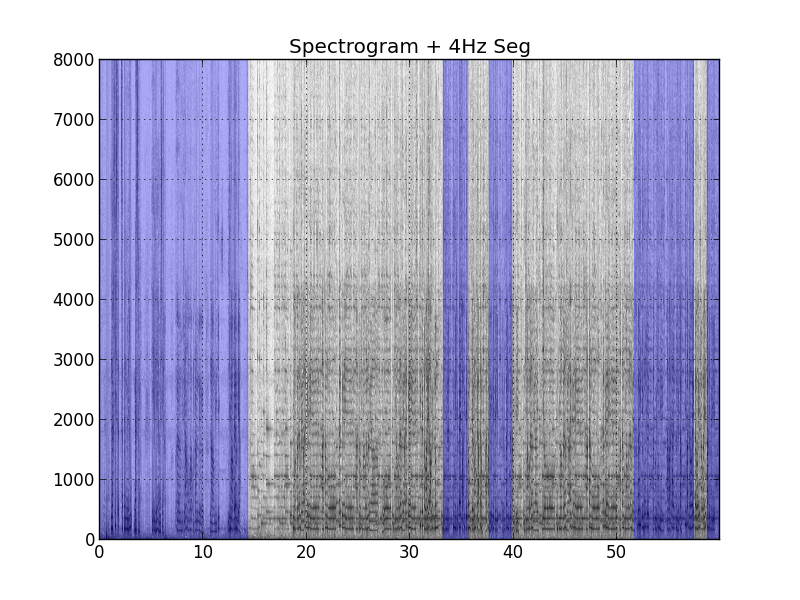
\includegraphics[width=0.8\linewidth]{img/irit_speech4hz}\\
\href{sounds/CNRSMH_I_2013_202_001_06.mp3}{CNRSMH\_I\_2013\_202\_001\_06}
\end{center}
\end{frame}
\begin{frame}\frametitle{Aubio Pitch + Aubio Beat}
  \begin{center}
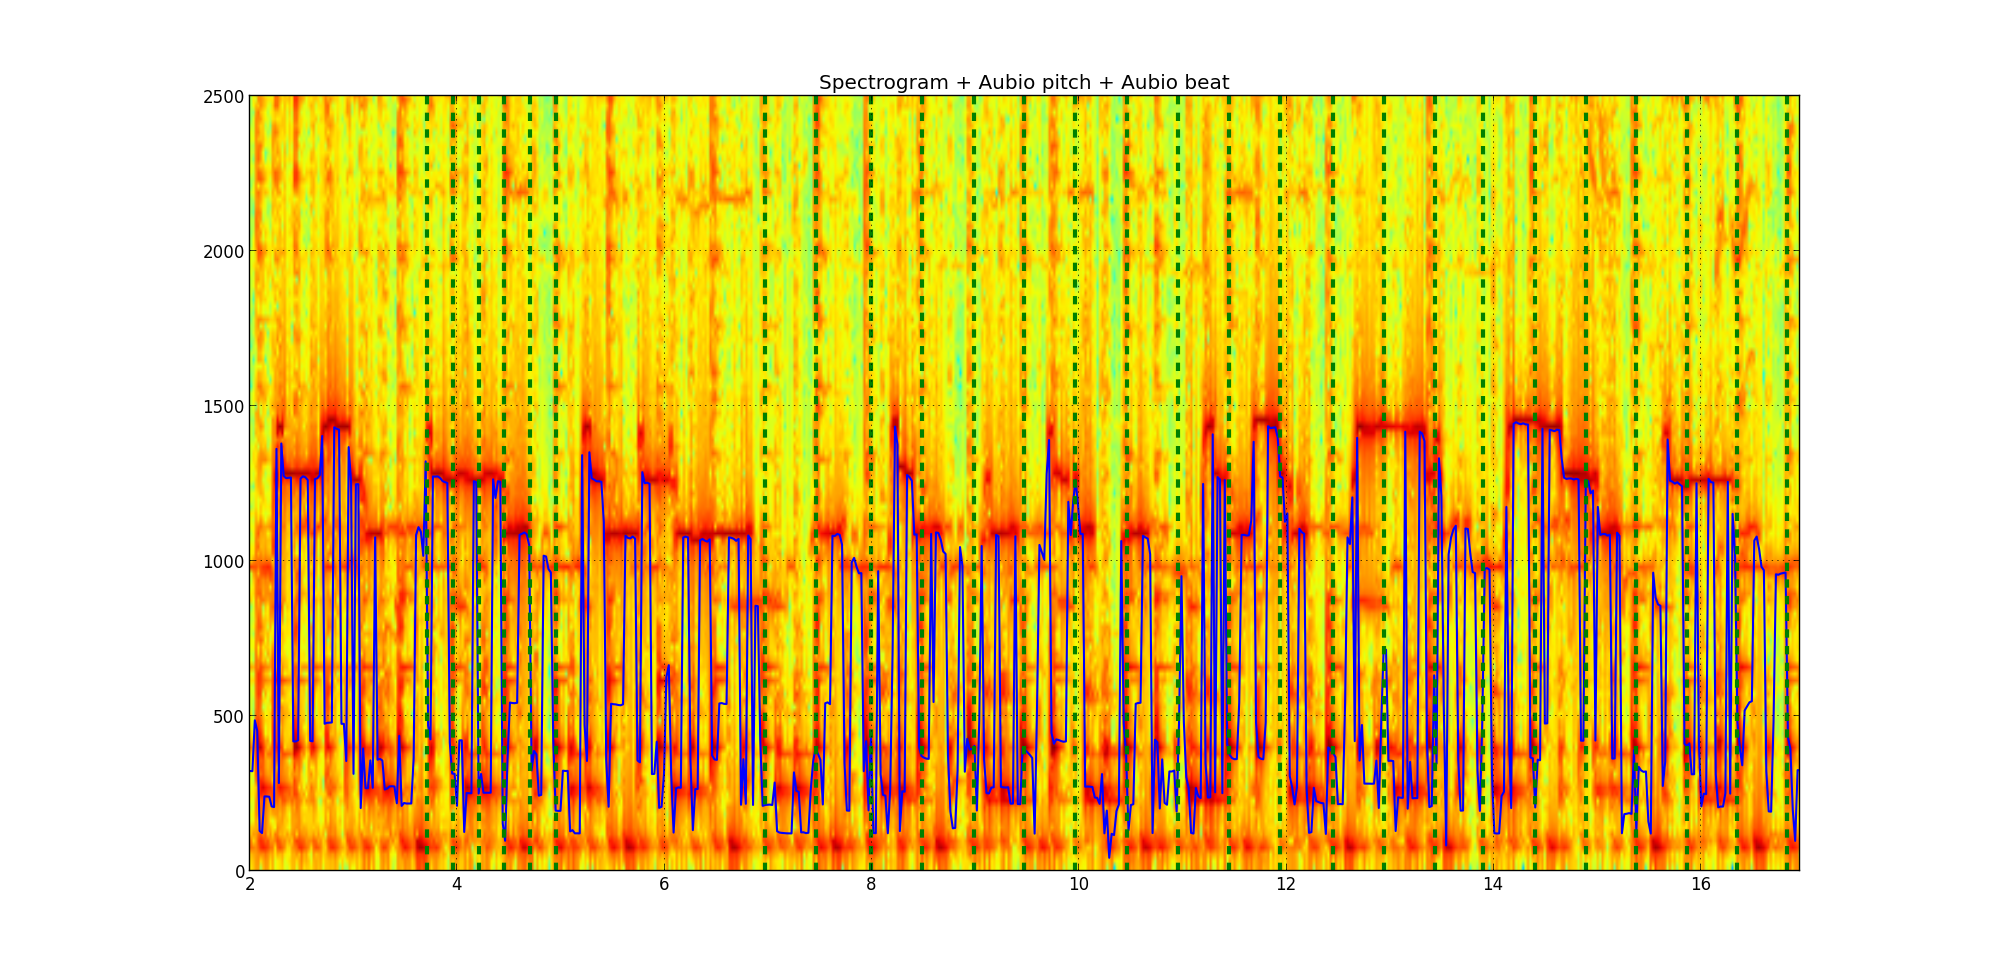
\includegraphics[width=1.1\linewidth]{img/aubio_pitch_beat.png}\\
\href{sounds/CNRSMH_E_1985_001_001_001_04.mp3}{CNRSMH\_E\_1985\_001\_001\_001\_04}
\end{center}
\end{frame}

\begin{frame}\frametitle{Telemeta Player Mark}
  \vspace{-1cm}
  \begin{center}
    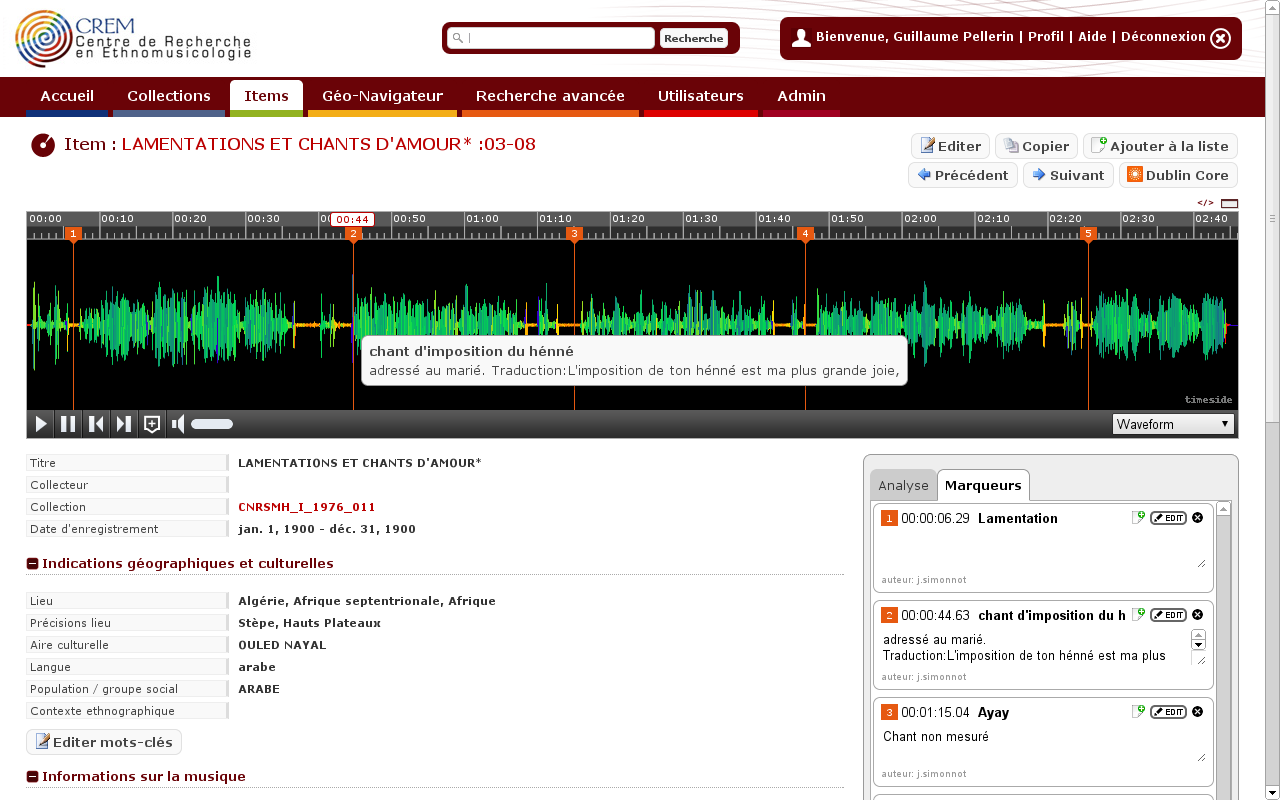
\includegraphics[width=12cm]{../../Common/img/shots/player_mark.png}
  \end{center}
\end{frame}

\begin{frame}
\frametitle{DIADEMS Project}
\begin{itemize}
\item ANR project: \emph{Description, Indexation, Accès aux Documents EthnoMusicologiques et Sonores} \\
(Description, Indexation, Access to Sound and Ethnomusicological Documents)\\
\url{http://www.irit.fr/recherches/SAMOVA/DIADEMS}
\item Partners:
  \begin{itemize}
  \item Ethnomusicology:
    \begin{itemize}
    \item CREM (Centre de Recherche en EthnoMusicologie),
      Univ. Nanterre
    \item MNHM (Museum National d'Histoire Naturelle)
    \end{itemize}
  \item Computer science, Music Informationa Retrieval, Speech Processing:
    \begin{itemize}
    \item IRIT, Toulouse
    \item LAM, Paris 6
    \item LIMSI, Orsay
    \item LABRI, Bordeaux
    \end{itemize}

  \end{itemize}

\end{itemize}
\end{frame}
\begin{frame}
\frametitle{Goals}
%\begin{block}{Thesaurus}
\begin{itemize}
\item Improvement of the Telemeta User Interface
\item Enhance annotation interface and management
\item Introduce automatic description, indexation, segmentation with music information retrieval, audio signal and speech processing technologies $\rightarrow$ \emph{TimeSide} 
\item Ethnomusicological metadata: \href{Thesaurus.html}{Thesaurus
    Map}
\end{itemize}

%\end{block}
\end{frame}
\begin{frame}
\frametitle{The End}
\begin{center}
  \LARGE Merci !
\end{center}
\end{frame}
\end{document}
%%% Local Variables: 
%%% mode: latex
%%% TeX-master: t
%%% End: 
